\chapter{Rezultate}

Rezultatele clasificatorilor pe setul de test au fost destul de mici, însă și faptul că sunt puține date
de clasă 1 în acest set influențează acest lucru. Astfel, sunt doar 263 de tweet-uri de clasă 1, care, poate
ar avea caracteristici diferite de tweet-urile din setul de antrenament. Din păcate nu am avut acces la 
setul de test oficial al concursului, care, din lucrarea celor de la echipa NRC-Canada, au fost 9961 de tweet-uri,
dintre care 771 de clasă 1. Ar fi fost de mare ajutor acest set de date, deoarece și pentru antrenare aș fi avut mai
multe tweet-uri de folosit. 

În graficul de mai jos se poate vedea diferența dintre rezultate, între cele două metode de transformare a textului 
în vectori folosite, Word2Vec și fasttext, și pe baza clasificatorilor folosiți. De precizat este că setul de antrenament
folosit este cel secționat la 70\%, după care i-a fost aplicat algoritmul SMOTE pentru balansarea acestuia, până când
datele de clasă 1 au devenit egale cu cele de clasă 0.

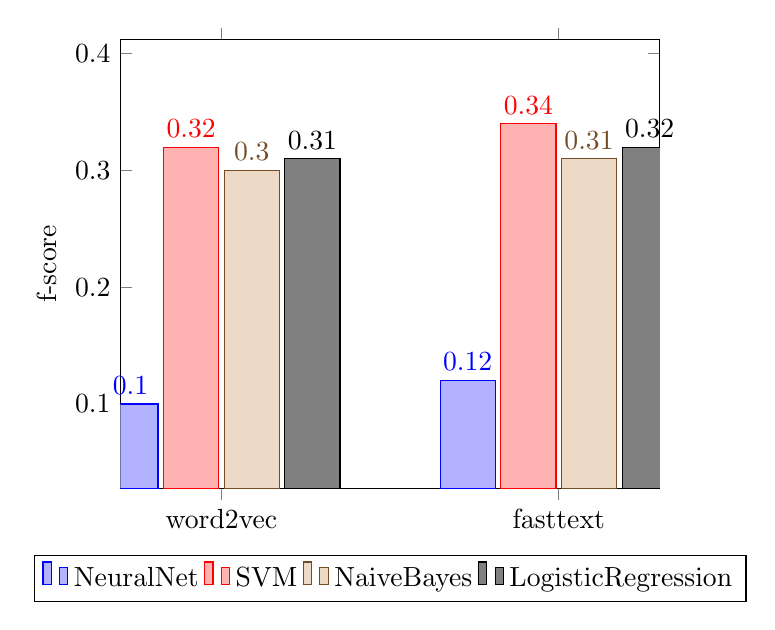
\begin{tikzpicture}
    \begin{axis}[
        ybar,
        bar width=0.7cm,
        enlargelimits=0.3,
        legend style={at={(0.5,-0.15)},
          anchor=north,legend columns=-1},
        ylabel={f-score},
        symbolic x coords={word2vec, fasttext},
        xtick=data,
        nodes near coords,
        nodes near coords align={vertical},
        ]
    \addplot coordinates {(word2vec, 0.1) (fasttext,0.12)};
    \addplot coordinates {(word2vec, 0.32) (fasttext,0.34)};
    \addplot coordinates {(word2vec, 0.3) (fasttext,0.31)};
    \addplot coordinates {(word2vec, 0.31) (fasttext,0.32)};
    \legend{NeuralNet, SVM, NaiveBayes, LogisticRegression}
\end{axis}
\end{tikzpicture}

Am considerat că acest grafic pune cel mai bine în valoare fiecare metodă, fiind folosită cea mai bună
metodă de balansare a datelor, celelalte metode nefiind la fel de eficiente.